\chapter{Additional results for score matching}

\section{Technical results}
\label{chap:Technical}

\subsection{Exact solution for the kernel denoising score matching with RFF}
\label{sec:exact_solution}
We start with the first-order optimality condition:
\begin{equation*}
    \int p_{\varepsilon}({\bf y}) A^*({\bf y})\nabla V(A({\bf y})f)d{\bf y} + \lambda f = 0,
\end{equation*}
where $A^*({\bf y}): \mathbb{R}^m \to \mathcal{H}$ is an adjoint to $A({\bf y})$ and
$A^*({\bf y}){\bm \alpha} = \sum_{i = 1}^m \alpha_i\phi_i({\bf y}, \cdot)$.
Denoting
\begin{align*}
    &{\bm \alpha}({\bf y}) = -\frac{1}{\lambda}\nabla V(A({\bf y})f),\quad f = \int p_{\varepsilon}({\bf y})A^*({\bf y}){\bm \alpha}({\bf y})d {\bf y},
\end{align*}
the first-order optimality condition could be rewritten as an integral equation on
${\bm \alpha}({\bf y})$:
\begin{equation}
    {\bm \alpha}({\bf y}) = -\frac{1}{\lambda}\nabla V\left(\int p_{\varepsilon}({\bf z})A({\bf y})A^*({\bf z})\alpha({\bf z})d{\bf z}\right),
\end{equation}
where $A({\bf y})A^*({\bf z})\alpha({\bf z}) = \sum\limits_{i = 1}^m\alpha_i({\bf z})\{\langle \phi_j({\bf y}, \cdot),  \phi_i({\bf z}, \cdot)\rangle\}_{j = 1}^m = {\bm K}({\bf y}, {\bf z}){\bm \alpha}({\bf z})$.

The gradient of $V$ is given
by~$\nabla V = (\frac{1}{n}, \frac{1}{n}, \ldots, \frac{1}{n}, 1)^{\top}$.
Then, we have ${\bm \alpha}({\bf y}) = ({\bm \beta}^{\top}({\bf y}), \delta)^{\top}$,
where $\delta = -\frac{1}{\lambda}$.
Therefore, the integral equation on ${\bm \beta}({\bf y})$ can be expressed as
\begin{equation}
    {\bm \beta}({\bf y}) = -\frac{1}{n\lambda}\int p_{\varepsilon}({\bf z})\hat{A}({\bf y})\hat{A}({\bf z})^*{\bm \beta}({\bf z})d{\bf z} + \frac{1}{n\lambda^2}\int p_{\varepsilon}({\bf z}) \hat{A}({\bf y}) \phi_m({\bf z}, \cdot)d{\bf z},
\end{equation}
where $(\hat{A}({\bf y})f)_i = (A({\bf y})f)_i$, $i = 1, \ldots, m - 1$.
Let $b = \int p_{\varepsilon}({\bf y})\phi_m({\bf y}, \cdot) d {\bf y}$ and
$C = \int p_{\varepsilon}({\bf y})\hat{A}^*({\bf y}){\bm \beta}({\bf y}) d {\bf y}$.
Next, we search for the solution of \eqref{eq:beta_integal} in the form
${\bm \beta}({\bf y}) = -\frac{1}{n\lambda}\hat{A}({\bf y})C + \frac{1}{n\lambda^2}\hat{A}({\bf y})b$.
In this case, we have
\begin{equation*}
    \hat{A}({\bf y})\left[C + \frac{1}{n\lambda}BC - \frac{1}{n\lambda^2}Bb\right] = 0,
\end{equation*}
where $B = \int p_{\varepsilon}({\bf y})\hat{A}^*({\bf y})\hat{A}({\bf y}) d{\bf y}$ and
$b \in \mathcal{H}$ is a convolution of $\phi_m$ and noise density $p_{\varepsilon}$.
% Indeed, fixing ${\bf z}$, $\phi_m({\bf y, z}) \in H$ as a function of ${\bf y}$. Then ${\cal F}[\phi_m({\bf y, z}) * p_{\varepsilon}({\bf y})] = {\cal F}[\phi_m({\bf y, z})]{\cal F}[p_{\varepsilon}({\bf y})]$.
% $$\int \frac{|{\cal F}[\phi_m({\bf y, z})]{\cal F}[p_{\varepsilon}({\bf y})]|^2}{{\cal F}[k](w)}dw \leq \sup|{\cal F}[p_{\varepsilon}({\bf y})]|^2\int \frac{|{\cal F}[\phi_m({\bf y, z})]|^2}{{\cal F}[k](w)}dw < \infty$$
% The last follow $p_{\varepsilon}({\bf y}) \in L^1$.

%As produnct of function from $H$ belongs to $H$
Solution $C^*$ of the above equation provides ${\bm \beta}^*({\bf y})$ and, as a result,
the solution to the initial problem.
Let us show that the obtained estimator belongs to $H$.
In fact, since
\[
    C + \frac{1}{n\lambda}BC - \frac{1}{n\lambda^2}Bb \in {\rm Ker}\hat{A}({\bf y}) \subseteq
    \mathcal{H}
\]
and $B + n\lambda I$ is continuously invertible, we have that $C^* \in \mathcal{H}$.
Finally, we have
\[
    f^* = B\left[-\frac{1}{n\lambda}C^* + \frac{1}{n\lambda^2}b\right] = C^* - \frac{1}{\lambda}b - \gamma \in \mathcal{H},
\]
where we assume $\gamma \in {\rm Ker}\hat{A}({\bf y})$.



\subsection{RFF solution derivation}
\label{sec:rff_solution_derivation}
Let us use the expressions for the solution without noise
(for simplicity, the term with $\partial_i \log q_0({\bf x}_a)$ is omitted here):
\begin{equation*}
    \left [ \hat{A}({\bf 0})\hat{A}({\bf 0})^* \right ]_{(a - 1)d + i, (b - 1)d + j} =
    \partial_i\partial_{j + d}k({\bf x}_a, {\bf x}_b),~\quad a, b \in [n],~i, j \in [d],
\end{equation*}
\begin{equation*}
    \left [ \hat{A}({\bf 0}){\bm \phi}_m({\bf 0}, \cdot) \right ]_{(a - 1)d + i} =
    \frac{1}{n}\sum_{b, j = 1}^{n, d}\partial_i\partial^2_{j + d}k({\bf x}_a, {\bf x}_b),~\quad a\in [n],~i \in [d].
\end{equation*}
Then we have
$\hat{A}({\bf y})\hat{A}({\bf z})^* \approx \partial{\bm \Phi}_y\partial{\bm \Phi}_z^{\top}$
and
$\hat{A}({\bf y}){\bm \phi}_m({\bf z}, \cdot) * p_{\varepsilon}({\bf z}) \approx \frac{1}{n}
\partial{\bm \Phi}_y(\partial^2{\bm \Phi}_z * p_{\varepsilon}({\bf z}))^{\top}{\bf 1}$.

Now, we can obtain the RFF approximation of \eqref{eq:beta_finite_sample}:
\begin{align*}
    {\bm \beta}_K = -\frac{1}{nK\lambda}\partial {\bm \Phi}_K\partial {\bm \Phi}_K^{\top}{\bm \beta}_K  + \frac{1}{n^2\lambda^2}\partial{\bm \Phi}_K \odot (\partial^2 {\bm \Phi}_z * p({\bf z}))^{\top}{\bf 1},
\end{align*}
where
\[  \partial {\bm \Phi}_K =
    \begin{bmatrix}
        {\bm \Phi}_{z_1}\\
        \vdots\\
        {\bm \Phi}_{z_K}
    \end{bmatrix}, \quad
    \partial{\bm \Phi}_K \odot (\partial^2 {\bm \Phi}_z * p({\bf z}))^{\top}{\bf 1} =
    \begin{bmatrix}
        \partial{\bm \Phi}_{z_1}(\partial^2 {\bm \Phi}_z * p({\bf z}))^{\top}{\bf 1}\\
        \vdots\\
        \partial{\bm \Phi}_{z_K}(\partial^2 {\bm \Phi}_z * p({\bf z}))^{\top}{\bf 1}
    \end{bmatrix}.
\]
Denoting
\begin{equation*}
    {\bm h} = \frac{1}{n}(\partial^2 {\bm \Phi}_z * p({\bf z}))^{\top}{\bf 1},
    \quad
    {\bm H} =
    \int p_{\varepsilon}({\bf y})\partial{\bm \Phi}_y^{\top}\partial{\bm \Phi}_y d{\bf y}
\end{equation*}
we obtain the following expression for the descretized solution $f_K$:
\begin{align*}
    f_K
    &= \frac{1}{n\lambda^2}{\bm \phi}(\cdot)^{\top}{\bm H} \left[-\frac{1}{K}\partial {\bm \Phi}_K^{\top}\left(\frac{1}{K}\partial {\bm \Phi}_K\partial {\bm \Phi}_K^{\top} + n\lambda {\bf I}\right)^{-1}\partial{\bm \Phi}_K \odot {\bm h} + {\bm h}\right]
   -\frac{1}{\lambda} {\bm \phi}(\cdot)^{\top}{\bm h}\\
    &= \frac{1}{n\lambda^2}{\bm \phi}(\cdot)^{\top}{\bm H}
    \left[-\frac{1}{K}\left(\frac{1}{K}\partial  {\bm \Phi}_K^{\top}\partial{\bm \Phi}_K + n\lambda {\bf I}\right)^{-1}\partial {\bm \Phi}_K^{\top}\partial{\bm \Phi}_K \odot {\bm h} + {\bm h}\right]
    -\frac{1}{\lambda} {\bm \phi}(\cdot)^{\top}{\bm h}.
\end{align*}
By taking a limit over $K \to \infty$, and using
${\bm H} = \lim\limits_{K \to \infty}\frac{1}{K}\partial {\bm \Phi}_K^{\top}\partial{\bm\Phi}_K$ along with
\begin{equation*}
    \lim\limits_{K \to \infty}(n\lambda{\bf I} + \frac{1}{K}\partial {\bm \Phi}^{\top}_K\partial {\bm \Phi}_K) \lim\limits_{K \to \infty}\frac{1}{K}\partial {\bm \Phi}^{\top}_K{\bm \beta}_K = \lim\limits_{K \to \infty}\frac{1}{K\lambda}\partial {\bm \Phi}^{\top}_K\partial {\bm \Phi}_K{\bm h},
\end{equation*}
the solution $f^*$ is given as
\begin{align*}
    f_{m}^* = \lim\limits_{K \to \infty} f_K
    &= -\frac{1}{n\lambda^2}{\bm\phi}(\cdot)^{\top}{\bm H}({\bm H} +
    n \lambda {\bf I})^{-1}{\bm Hh} + \frac{1}{n\lambda^2}{\bm \phi}(\cdot)^{\top}{\bm Hh} -
    \frac{1}{\lambda}{\bm \phi}(\cdot)^{\top}{\bm h}\nonumber\\
    &= \frac{1}{\lambda}{\bm \phi}(\cdot)^{\top}({\bm H} + n\lambda{\bf I})^{-1}{\bm Hh}
    - \frac{1}{\lambda}{\bm \phi}(\cdot)^{\top}{\bm h},
\end{align*}
where index $m$ refers to the number of RFF features.




\subsection{Proof for the error bounds of score matching with RFF}
\label{sec:error_bound_proof}
The idea of this proof is to upper bound the expected square difference between solutions:
\begin{equation}
    \mathbb{E}_{{\bf x}, {\bf w}}(f_{n, m}^*({\bf x}) - f_n^*({\bf x}))^2,
\end{equation}
where the difference between RFF and exact kernel solutions ($f_{n, m}^*,~f_n^*$)
is expressed as follows:
\begin{align*}
    f_{n, m}^* - f_n^*
    &= -\frac{1}{\lambda n}\partial^2{\bm k}(\cdot)^{\top}{\bf 1}
    + \frac{1}{\lambda n} {\bm \phi}^{\top}(\cdot)\partial^2\bm{\Phi}^{\top}{\bf 1} \\
    &+ \frac{1}{\lambda n}\partial{\bm k}(\cdot)^{\top}(\partial\partial {\bm K} +
    \lambda n{\bf I})^{-1}\partial\partial^2 {\bm K}{\bf 1}
    -\frac{1}{\lambda n}{\bm \phi}^{\top}(\cdot)\partial\bm{\Phi}^{\top}(\partial\bm{\Phi}
    \partial\bm{\Phi}^{\top} +
    \lambda n {\bf I})^{-1}\partial\bm{\Phi}\partial^2\bm{\Phi}^{\top}{\bf 1} \\
    &= \frac{1}{\lambda n}(\partial^2\bm{\Phi}{\bm \phi}(\cdot) -
    \partial^2{\bm k}(\cdot))^{\top}{\bf 1}
    + \frac{1}{\lambda n}(\partial{\bm k}(\cdot) -
    \partial\bm{\Phi}{\bm \phi}(\cdot))^{\top}(\partial\partial {\bm K} +
    \lambda n{\bf I})^{-1}\partial\partial^2 {\bm K}{\bf 1} \\
    &+ \frac{1}{\lambda n}{\bm \phi}^{\top}(\cdot)\partial\bm{\Phi}^{\top} \left[
        (\partial\partial {\bm K} + \lambda n{\bf I})^{-1} -
        (\partial\bm{\Phi}\partial\bm{\Phi}^{\top} + \lambda n {\bf I})^{-1}
    \right] \partial\partial^2 {\bm K}{\bf 1} \\
    &+ \frac{1}{\lambda n}{\bm \phi}^{\top}(\cdot)\partial\bm{\Phi}^{\top}(\partial\bm{\Phi}
    \partial\bm{\Phi}^{\top} + \lambda n {\bf I})^{-1}(\partial\partial^2 {\bm K} -
    \partial\bm{\Phi}\partial^2\bm{\Phi}^{\top}){\bf 1}.
\end{align*}
The above expectation is taken jointly over random Fourier weights and given points
${\bf x} \sim p_0$.
It can then be written as
$\mathbb{E}_{{\bf x}, {\bf w}}[f] = \mathbb{E}_{{\bf w}}\mathbb{E}_{{\bf x}}[f | {\bf w}]$.
The first term in the above expression is the difference between $\hat{\xi}$
and its RFF approximation $\hat{\xi}_m$, so, we have:
\begin{align*}
    \mathbb{E}_{{\bf w}}{\bf 1}^{\top}&(\partial^2\bm{\Phi}{\bm \phi}(\cdot) - \partial^2{\bm k}(\cdot))(\partial^2\bm{\Phi}{\bm \phi}(\cdot) - \partial^2{\bm k}(\cdot))^{\top}{\bf 1} \\
    &= {\bf 1}^{\top}\left[\mathbb{E}_{{\bf w}}[\partial^2\bm{\Phi}{\bm \phi}(\cdot){\bm \phi}(\cdot)^{\top}\partial^2\bm{\Phi}^{\top}] - \partial^2{\bm k}(\cdot)\partial^2{\bm k}(\cdot)^{\top}\right]{\bf 1}\\
    &\leq \frac{m - 1}{m}{\bf 1}^{\top}\partial^2{\bm k}(\cdot)\partial^2{\bm k}^{\top}(\cdot){\bf 1} + \frac{1}{m}{\bf 1}^{\top}\partial^2\partial^2{\bm K}{\bf 1} - {\bf 1}^{\top}\partial^2{\bm k}(\cdot)\partial^2{\bm k}(\cdot)^{\top}{\bf 1}\\
    &\leq \frac{1}{m}{\bf 1}^{\top}\partial^2\partial^2{\bm K}{\bf 1},
\end{align*}
where the first inequality is obtained using
$\sup_{\bf x}|\phi_i({\bm W}{\bf x} + {\bm b})| \leq 1$.
As this expression does not depend on ${\bf x}$, the joint expectation will be the same.

For the second term in $f_{n, m}^*({\bf x}) - f_n^*({\bf x})$, derivation of the
upper bound is technically the same, but with lower-order derivatives, so
\begin{align*}
    \mathbb{E}_{{\bf w}}\left[(\partial{\bm k}(\cdot) -
    \partial\bm{\Phi}{\bm \phi}(\cdot))^{\top}(\partial\partial {\bm K} +
    \lambda n{\bf I})^{-1}\partial\partial^2 {\bm K}{\bf 1}\right]^2 \leq \\
    \frac{1}{m}\|\partial\partial {\bm K}^{\frac{1}{2}}(\partial\partial {\bm K} + \lambda n{\bf I})^{-1}\partial\partial^2 {\bm K}{\bf 1}\|^2.
\end{align*}

The third them is
\begin{align*}
    \mathbb{E}_{{\bf x, w}}&\left[{\bm \phi}^{\top}(\cdot)\partial\bm{\Phi}^{\top}\left[(\partial\partial {\bm K} + \lambda n{\bf I})^{-1} - (\partial\bm{\Phi}\partial\bm{\Phi}^{\top} + \lambda n {\bf I})^{-1}\right]\partial\partial^2 {\bm K}{\bf 1}\right]^2 \\
    &= \mathbb{E}_{{\bf x, w}}\left[{\bm \phi}^{\top}(\cdot)\partial\bm{\Phi}^{\top}(\partial\bm{\Phi}\partial\bm{\Phi}^{\top} + \lambda n{\bf I})^{-1}(\partial\partial {\bm K} - \partial\bm{\Phi}\partial\bm{\Phi}^{\top})(\partial\partial {\bm K} + \lambda n {\bf I})^{-1}\partial\partial^2 {\bm K}{\bf 1}\right]^2\\
    &\leq \mathbb{E}_{{\bf w}}\mathbb{E}_{{\bf x}}\left[\|{\bf R}\|_2 \|(\partial\partial {\bm K} - \partial\bm{\Phi}\partial\bm{\Phi}^{\top})(\partial\partial {\bm K} + \lambda n {\bf I})^{-1}\partial\partial^2 {\bm K}{\bf 1}\|^2 | {\bf w}\right],
\end{align*}
where only $\bf R$ depends on ${\bf x}$.
\begin{align*}
    \mathbb{E}_{\bf x}{\bf R}
    &= (\partial\bm{\Phi}\partial\bm{\Phi}^{\top} + \lambda n{\bf I})^{-1}\partial\bm{\Phi}
    \mathbb{E}_{\bf x}\left[{\bm \phi}(\cdot){\bm \phi}^{\top}(\cdot)\right]\partial\bm{\Phi}^{\top}(\partial\bm{\Phi}\partial\bm{\Phi}^{\top} + \lambda n{\bf I})^{-1}\\
    &= \frac{1}{n} (\partial\bm{\Phi}\partial\bm{\Phi}^{\top} + \lambda n{\bf I})^{-1}\partial\bm{\Phi}
    (\bm{\Phi}^{\top}\bm{\Phi} + \varepsilon n I)\partial\bm{\Phi}^{\top}(\partial\bm{\Phi}\partial\bm{\Phi}^{\top} + \lambda n{\bf I})^{-1}
\end{align*}
This inequality holds with the probability $1 - \delta$ for
$n \geq \frac{8}{3\varepsilon^2} \log\frac{m}{\delta}$
%$n \geq \frac{8 \sup_{\bf x}k({\bf x}, {\bf x})}{3\varepsilon^2} \log\frac{m}{\delta}$
and is obtained from the Bernstein inequality assuming that the weights are fixed \cite{Tropp_2015}.
\begin{align*}
    \lambda_{\max}({\bf R})
    &= \frac{1}{n}\lambda_{\max}\left[(\partial\bm{\Phi}\partial\bm{\Phi}^{\top} +
    \lambda n{\bf I})^{-1}\partial\bm{\Phi}
    (\bm{\Phi}^{\top}\bm{\Phi} + n\varepsilon I)\partial\bm{\Phi}^{\top}(\partial\bm{\Phi}
    \partial\bm{\Phi}^{\top} + \lambda n{\bf I})^{-1}\right]\\
    &\leq \frac{1}{n}\lambda_{\max}\left[(\bm{\Phi}^{\top}\bm{\Phi} + n\varepsilon I)
    \partial\bm{\Phi}^{\top}(\partial\bm{\Phi}\partial\bm{\Phi}^{\top} + \lambda n{\bf I})^{-1}\partial\bm{\Phi}
    \right]\\
    &\leq \frac{1}{n}\lambda_{\max}\left[(\bm{\Phi}^{\top}\bm{\Phi} + n\varepsilon I)\right] \leq
    \frac{1}{n}{\rm tr}\left[(\bm{\Phi}^{\top}\bm{\Phi} + n\varepsilon I)\right] \\
    &\leq \left(\frac{1}{m}\max_i\sup_{\bf x}\|\phi_i({\bm W}{\bf x} + {\bm b})\|^2 +
    \varepsilon\right) \leq \frac{1}{m} + \varepsilon
\end{align*}
\begin{align*}
    \mathbb{E}_{\bf w}&\|(\partial\partial {\bm K} - \partial\bm{\Phi}\partial\bm{\Phi}^{\top})(\partial\partial {\bm K} + \lambda n {\bf I})^{-1}\partial\partial^2 {\bm K}{\bf 1}\|^2\\
    & = {\bf 1}^{\top}\partial\partial^2 {\bm K}^{\top}(\partial\partial {\bm K} + \lambda n {\bf I})^{-1}(\mathbb{E}_{\bf w}\partial\bm{\Phi}\partial\bm{\Phi}^{\top}\partial\bm{\Phi}\partial\bm{\Phi}^{\top} - \partial\partial {\bm K}^2)(\partial\partial {\bm K} + \lambda n {\bf I})^{-1}\partial\partial^2 {\bm K}{\bf 1}
\end{align*}
\begin{align*}
    \mathbb{E}_{\bf w}\partial\bm{\Phi}\partial\bm{\Phi}^{\top}\partial\bm{\Phi}\partial\bm{\Phi}^{\top} = \frac{m - 1}{m} \partial\partial {\bm K}^2 + \frac{1}{m}{\bf D}_1.
\end{align*}
The latter term here is obtained under the assumption that ${\bf D}_1$ does not depend on
${\bf x}$.
This assumption holds for sufficiently smooth kernels and we can
rewrite the expression under an expectation as the polynomial of weights times
the trigonometric function.
\begin{align*}
    \mathbb{E}_{\bf w}&\|(\partial\partial {\bm K} - \partial\bm{\Phi}\partial\bm{\Phi}^{\top})(\partial\partial {\bm K} + \lambda n {\bf I})^{-1}\partial\partial^2 {\bm K}{\bf 1}\|^2
    \leq \frac{1}{m}\|{\bf D}_1^{\frac{1}{2}}(\partial\partial {\bm K} + \lambda n {\bf I})^{-1}\partial\partial^2 {\bm K}{\bf 1}\|^2
\end{align*}
Analogously, for the last term, using the assumption that ${\bf D}_2 < \infty$, we have
\begin{align*}
    \mathbb{E}_{{\bf x, w}} \partial\bm{\Phi}\partial^2\bm{\Phi}^{\top}\partial\bm{\Phi}\partial^2\bm{\Phi}^{\top} \leq \frac{1}{m}\|{\bf D}_2^{\frac{1}{2}}{\bf 1}\|^2.
\end{align*}

Finally, combining all the above, we have
\begin{align*}
    \mathbb{E}_{{\bf x}, {\bf w}}(f_{n, m}^*({\bf x}) - f_n^*({\bf x}))^2 \leq \frac{2}{\lambda^2 n^2 m^2}\left[
    m{\bf 1}^{\top}\partial^2\partial^2{\bm K}{\bf 1} + m\|\partial\partial {\bm K}^{\frac{1}{2}}(\partial\partial {\bm K} + \lambda n{\bf I})^{-1}\partial\partial^2 {\bm K}{\bf 1}\|^2 \right. \nonumber \\
    \left. + (1 + \varepsilon m)\|{\bf D}_2^{\frac{1}{2}}{\bf 1}\|^2 + (1 + \varepsilon m)\|{\bf D}_1^{\frac{1}{2}}(\partial\partial {\bm K} + \lambda n {\bf I})^{-1}\partial\partial^2 {\bm K}{\bf 1}\|^2
    \right].
\end{align*}



\subsection{Derivation of \texorpdfstring{${\bm H}$ and ${\bm h}$ for }
 GGaussian noise}
\label{sec:Hh_der}
    \begin{align*}
        {\bm H}
        &= \partial \Phi^{\top}\partial \Phi * p_{\varepsilon}\\
        &= \sum\limits_{a = 1}^n\sum\limits_{i = 1}^d \partial_i \phi(\bm{W}{\bf x}_a + \bm{b})\partial_i \phi^{\top}(\bm{W}{\bf x}_a + \bm{b}) * p_{\varepsilon}\\
        &= \sum\limits_{a = 1}^n\sum\limits_{i = 1}^d \bm{W}_{:, i}\bm{W}_{:, i}^\top \odot \phi'(\bm{W}{\bf x}_a + \bm{b}) \phi'^\top(\bm{W}{\bf x}_a + \bm{b}) * p_{\varepsilon}\\
        &= \frac{1}{M}\bm{W}\bm{W}^{\top} \odot \sum\limits_{a = 1}^n \sin(\bm{W}{\bf x}_a + \bm{b}) \sin^\top(\bm{W}{\bf x}_a + \bm{b}) * p_{\varepsilon}
        \label{eq:H_derivation}
    \end{align*}
    Assuming that $p_{\varepsilon} = {\cal N}({\bf 0}, \sigma^2{\bf I})$ and using
    \begin{align*}
        \cos(\mathbf{w}^\top \mathbf{x}) * \mathcal{N}(0, \sigma^2\mathbf{I}) &=
        %\int_\mathbf{y} \cos(\mathbf{w}^\top(\mathbf{x} - \mathbf{y}))
        %\frac{\exp\left(-\frac{\|\mathbf{y}\|^2}{2\sigma^2}\right )}{Z} d\mathbf{y}
         e^{-\frac{\sigma^2}{2}\|\mathbf{w}\|_2^2}\cos(\mathbf{w}^\top \mathbf{x}),
    \end{align*}
    we will obtain
    \begin{align*}
        \sin(\mathbf{w^\top x} + b) \sin(\mathbf{v^\top x} + c) * p_{\varepsilon}
        &= \frac{1}{2}\left[\cos ((\mathbf{w - v})^\top \mathbf{x} + b - c) - \cos ((\mathbf{w + v} + b + c)^\top \mathbf{x})\right] * p_{\varepsilon}\\
        &= \frac{1}{2}e^{-\frac{\sigma^2}{2}\|\mathbf{w - v}\|_2^2}\cos ((\mathbf{w - v})^\top \mathbf{x} + b - c)\\
        &- \frac{1}{2}e^{-\frac{\sigma^2}{2}\|\mathbf{w + v}\|_2^2}\cos ((\mathbf{w + v})^\top \mathbf{x} + b + c)
    \end{align*}
    \begin{align}
        {\bm H} = \frac{1}{2M}\bm{W}\bm{W}^{\top} \odot \sum\limits_{a = 1}^n\left[
            e^{-\frac{\sigma^2}{2}\|{\bf w}_i - {\bf w}_j\|_2^2}\cos (({\bf w}_i - {\bf w}_j)^\top \mathbf{x}_a + {\bf b}_i - {\bf b}_j)
            \right .\nonumber \\
            \left .
            - e^{-\frac{\sigma^2}{2}\|{\bf w}_i + {\bf w}_j\|_2^2}\cos (({\bf w}_i + {\bf w}_j)^\top \mathbf{x}_a + {\bf b}_i + {\bf b}_j).
        \right]
    \end{align}
    Next, firstly assume that $q_0$ is uniform:
    \begin{align*}
        {\bm h}
        &= \frac{1}{n}\sum_{a = 1}^n\sum_{i = 1}^d \partial_i^2 \phi(\bm{W}{\bf x}_a + \bm{b}) * p_{\varepsilon}\\
        &= -\frac{1}{n\sqrt{M}}\sum_{a = 1}^n\sum_{i = 1}^d \bm{W}_{:, i}^2 \odot \cos(\bm{W}{\bf x}_a + \bm{b}) * p_{\varepsilon}\\
        &= -\frac{1}{n\sqrt{M}}\sum_{a = 1}^n {\rm diag}(\bm{W}\bm{W}^{\top})\odot e^{-\frac{\sigma^2}{2}{\rm diag}(\bm{W}\bm{W}^{\top})} \odot \cos(\bm{W}{\bf x}_a + \bm{b})
    \end{align*}
    For a multivariate normal $q_0(\bf x) = {\cal N}({\bm \mu} and {\bm \Sigma})$, $\nabla\log q_0(\bf x) = -{\bm \Sigma}^{-1}({\bf x} - {\bm \mu})$, there will be additional term to ${\bm h}$:
    \begin{align*}
        {\bm h}
        &= \frac{1}{n}\sum_{a = 1}^n\sum_{i = 1}^d \partial_i \phi(\bm{W}{\bf x}_a + \bm{b})\partial_i \log q_0({\bf x}_a) * p_{\varepsilon}\\
        &= -\frac{1}{n\sqrt{M}}\sum_{a = 1}^n\sum_{i = 1}^d \bm{W}_{:, i}\sin(\bm{W}{\bf x}_a + \bm{b})\partial_i \log q_0({\bf x}_a) * p_{\varepsilon}\\
        &= -\frac{1}{n\sqrt{M}} \sum_{a = 1}^n \sin(\bm{W}{\bf x}_a + \bm{b}) \odot \bm{W} \nabla\log q_0({\bf x}_a) * p_{\varepsilon}.
    \end{align*}
    Using
    \begin{align*}
    \mathbf{w}^\top {\bm \Sigma}^{-1}(\mathbf{x} - {\bm \mu}) \sin (\mathbf{w}^\top \mathbf{x}) * p_{\varepsilon}
    &=
    e^{-\frac{\sigma^2 \|\mathbf{w}\|^2}{2}}
    \mathbf{w}^\top{\bm \Sigma}^{-1}\left [
        (\mathbf{x} - {\bm \mu})\sin(\mathbf{w}^\top \mathbf{x}) + \sigma^2 \mathbf{w}\cos(\mathbf{w}^\top \mathbf{x})
    \right ],
    \end{align*}
    we obtain
    \begin{align}
        {\bm h} = \frac{1}{n\sqrt{M}}e^{-\frac{\sigma^2}{2}{\rm diag}(\bm{W}\bm{W}^{\top})} \odot \sum_{a = 1}^n \left[\sin(\bm{W}{\bf x}_a + \bm{b}) \odot {\bm W}{\bm \Sigma}^{-1}({\bf x}_a - {\bm \mu})
        \right . \nonumber\\
        \left .
        + \sigma^2\cos(\bm{W}{\bf x}_a + \bm{b})\odot {\rm diag}(\bm{W}{\bm \Sigma}^{-1}\bm{W}^{\top})
        \right]
    \end{align}
    In the case of arbitrary $q_0$, we use the Taylor expansion:
    \begin{equation*}
        \nabla \log q_0(\mathbf{x} + {\bm \varepsilon}) \approx
        \nabla \log q_0(\mathbf{x}) + \nabla^2 \log q_0(\mathbf{x}) {\bm \varepsilon}
    \end{equation*}
    In the vicinity of $\mathbf{x}$, it is equivalent to the previous case and the additional term is obtained with a simple replacement: $-{\bm \Sigma}^{-1} \to \nabla^2 \log q_0(\mathbf{x})$ and $-{\bm \Sigma}^{-1}({\bf x} - {\bm \mu}) \to \nabla \log q_0(\mathbf{x})$.

\subsection{Derivation of \texorpdfstring{$\bm H$ and $\bm h$
for arc-cosine kernels}.}
\label{sec:Hh_arccos}
\begin{align*}
        {\bm H}
        &= \partial \Phi^{\top}\partial \Phi * p_{\varepsilon}\\
        &= \sum\limits_{a = 1}^n\sum\limits_{i = 1}^d \partial_i \phi(\bm{W}{\bf x}_a)\partial_i \phi^{\top}(\bm{W}{\bf x}_a) * p_{\varepsilon}\\
        &= \sum\limits_{a = 1}^n\sum\limits_{i = 1}^d \bm{W}_{:, i}\bm{W}_{:, i}^\top \odot {\bf 1}(\bm{W}{\bf x}_a) \odot p^2(\bm{W}{\bf x}_a)^{p - 1}\left((\bm{W}{\bf x}_a)^{p - 1}\right)^{\top} * p_{\varepsilon}\\
        \label{eq:H_derivation}
    \end{align*}
    Considering $p = 2$, with uniform base density $q_0$ and isotropic Gaussian noise, we will obtain:
    \begin{align*}
        \bm{W}{\bf x}_a{\bf x}_a^{\top}\bm{W}^{\top} * p_{\varepsilon}
        & = \bm{W}\mathbb{E}_{p_{\varepsilon}}({\bf x}_a + {\bm \varepsilon})({\bf x}_a + {\bm \varepsilon})^{\top}\bm{W}^{\top} * p_{\varepsilon} = \bm{W}({\bf x}_a{\bf x}_a^{\top} + \sigma^2{\bf I})\bm{W}^{\top}
    \end{align*}
    The same holds for any symmetric noise distribution with covariance ${\bm \Sigma}$ and corresponding substitution to the above equation.
    \begin{equation}
        {\bm H} = 4\bm{W}\bm{W}^{\top} \odot \sum_{a = 1}^n{\bf 1}(\bm{W}{\bf x}_a) \odot \bm{W}({\bf x}_a{\bf x}_a^{\top} + \sigma^2{\bf I})\bm{W}^{\top}
    \end{equation}
    Moving to the computation of ${\bm h}$, we have:
    \begin{align*}
        {\bm h}
        &= \frac{1}{n}\sum_{a = 1}^n\sum_{i = 1}^d \partial_i^2 \phi(\bm{W}{\bf x}_a) * p_{\varepsilon}\\
        &= \frac{2}{n}\sum_{a = 1}^n\sum_{i = 1}^d \bm{W}_{:, i}^2 \odot {\bf 1}(\bm{W}{\bf x}_a) \odot (\bm{W}{\bf x}_a) * p_{\varepsilon}\\
        &= \frac{2}{n}{\rm diag}(\bm{W}\bm{W}^{\top}) \odot \sum_{a = 1}^n {\bf 1}(\bm{W}{\bf x}_a) \odot (\bm{W}{\bf x}_a),
    \end{align*}
    where the last line holds for any symmetric zero-mean density.

%\newpage
\subsection{The Taylor approximation of denoising score-matching}
\label{sec:Taylor}
    Considering the data corrupted by a small Gaussian noise $\hat{\mathbf{x}} = \mathbf{x} + {\bm \varepsilon}$, ${\bm \varepsilon}\sim {\cal N}(\mathbf{0}, \sigma^2 \mathbf{I})$ and by applying the Taylor expansion to the model density $p_m$, we obtain
    %, $s_m(x, \theta) = \nabla_x\log p_m(x, \theta)$
    %\begin{align*}
    %    J_{\varepsilon}(\theta) = \EE_{p_d}\EE_{\varepsilon}\left[{\rm tr}(\nabla_x s_m(\hat{x}, \theta)) + \frac{1}{2}\|s_m(\hat{x}, \theta)\|_2^2\right]
    %\end{align*}
    %\begin{align*}
    %    p_m(x + \varepsilon, \theta) = p_m(x, \theta) + \nabla_x p_m(x, \theta)^{\top} \varepsilon + \frac{1}{2}\varepsilon^{\top}\nabla^2_xp_m(x, \theta)\varepsilon + O(\|\varepsilon\|^3)
    %\end{align*}
    \begin{align*}
        \log p_m(\mathbf{x} + {\bm \varepsilon}, {\bm \theta}) = \log p_m(\mathbf{x}, {\bm \theta}) + \nabla\log p_m(\mathbf{x}, {\bm \theta})^{\top}{\bm \varepsilon} + \frac{1}{2}{\bm \varepsilon}^{\top}\nabla^2\log p_m(\mathbf{x}, {\bm \theta})^{\top}{\bm \varepsilon} + O(\|{\bm \varepsilon}\|_2^3),
    \end{align*}
    where ${\bm \theta}$ denotes a vector of model parameters, $\mathbb{E}[\varepsilon] = {\bf 0}$, $\mathbb{E}[\varepsilon\varepsilon^{\top}] = \sigma^2 {\bf I}$.
    %Assume $\nabla_x^i \EE [\cdots] = \EE \nabla^i_x (\cdots)$, $i = 1, 2$.
    \begin{align*}
        \mathbb{E}_{{\bm \varepsilon}}[\Delta_x\log p_m(\mathbf{x} + {\bm \varepsilon}, {\bm \theta})]
        &\approx \Delta_x \log p_m(\mathbf{x}, {\bm \theta}) + \frac{\sigma^2}{2}\Delta^2_x \log p_m(\mathbf{x}, {\bm \theta})
    \end{align*}
    \begin{align*}
        \|\nabla_x\log p_m(\mathbf{x} + {\bm \varepsilon}, {\bm \theta})\|_2^2
        &=\|\nabla_x\log p_m(\mathbf{x}, {\bm \theta})\|_2^2
        + 2\nabla_x\log p_m(\mathbf{x}, {\bm \theta})^{\top}\nabla_x^2\log p_m(\mathbf{x}, {\bm \theta}){\bm \varepsilon}\\
        &+ {\bm \varepsilon}^{\top}\nabla_x^2\log p_m(\mathbf{x}, {\bm \theta})^{\top}\nabla_x^2\log p_m(\mathbf{x}, {\bm \theta}){\bm \varepsilon}\\
        &+ \nabla_x\log p_m(\mathbf{x}, {\bm \theta})^{\top}\nabla_x{\bm \varepsilon}^{\top}\nabla_x^2\log p_m(\mathbf{x}, {\bm \theta}){\bm \varepsilon} + O(\|{\bm \varepsilon}\|_2^3)
    \end{align*}
    \begin{align*}
        \mathbb{E}_{{\bm \varepsilon}} \|\nabla_x\log p_m(\mathbf{x} + {\bm \varepsilon}, {\bm \theta})\|_2^2
        &\approx \|\nabla_x\log p_m(\mathbf{x}, {\bm \theta})\|_2^2 + \sigma^2{\rm tr}\left[\nabla_x^2\log p_m(\mathbf{x}, {\bm \theta})^{\top}\nabla_x^2log p_m(\mathbf{x}, {\bm \theta})\right] \\
        &+ \sigma^2 \nabla_x\log p_m(\mathbf{x}, {\bm \theta})^{\top}\nabla_x\Delta_x\log p_m(\mathbf{x}, {\bm \theta})
    \end{align*}
    Finally, we have
    \begin{align*}
        J_{{\bm \varepsilon}}({\bm \theta})
        &= J({\bm \theta}) + \frac{\sigma^2}{2}\mathbb{E}_{p_0}\left[(\Delta_x)^2 \log p_m(\mathbf{x}, {\bm \theta})\right]
       + \mathbb{E}_{p_0}{\rm tr}\left[\nabla_x^2\log p_m(\mathbf{x}, {\bm \theta})^{\top}\nabla_x^2\log p_m(\mathbf{x}, {\bm \theta})\right] \\
        &+ \mathbb{E}_{p_0}\left[\nabla_x\log p_m(\mathbf{x}, {\bm \theta})^{\top}\nabla_x\Delta_x\log p_m(\mathbf{x}, {\bm \theta})\right]
    \end{align*}
    where $p_0$ corresponds to an unknown data distribution.
    %$\nabla\log g(x + \varepsilon) = -\Sigma^{-1}(x + \varepsilon - \mu)$
    %\begin{align*}
    %    \nabla\log p(x + \varepsilon)^{\top}\nabla\log g(x + \varepsilon)
    %    \approx -(\nabla\log p(x) + \frac{\gamma}{2}\nabla\Delta \log p(x))^{\top}\Sigma^{-1}(x - \mu) - \gamma{\rm tr}\nabla^2\log p(x)\Sigma^{-1}
    %\end{align*}
    %Let $H = \left[\nabla_xs_m(x, \theta) - s_m(x, \theta)s_m(x, \theta)^{\top}\right]$
    %\begin{align*}
    %    J_{\varepsilon}(\theta) &\approx J(\theta) + \frac{\gamma}{2}\EE_{p_d}\left[\Delta_x{\rm tr}H + {\rm tr}H^{\top}H\right]
    %\end{align*}
%\newpage
\subsection{The Nystr\"{o}m kernel approximation}
\label{sec:Nystrom}
Let ${\bm K}$ be a sample Gram matrix, then for the Nystr\"{o}m kernel approximation \cite{Chen2016ErrorAO}, we have:
\[
    {\bm K} =
    \begin{bmatrix}
        {\bm K}_{11} & {\bm K}_{12}\\
        {\bm K}_{12}^{\top} & {\bm K}_{22}
    \end{bmatrix}
    \quad
    {\bm K} \approx
    \begin{bmatrix}
        {\bm K}_{11}\\
        {\bm K}_{12}^{\top}
    \end{bmatrix}
    {\bm K}_{11}^{-1}
    \begin{bmatrix}
        {\bm K}_{11} & {\bm K}_{12}
    \end{bmatrix}
    \quad
    \phi(x) =
    {\bm K}_{11}^{-\frac{1}{2}}{\bm k}({\bf x})
\]
where ${\bm k}({\bf x}) = \begin{bmatrix} {\bm k}({\bf x}, {\bf x}_1) & \ldots & {\bm k}({\bf x} and {\bf x}_M)\end{bmatrix}^{\top}$, $M$ is the amount of subsampled points.
\[
    \partial {\bm K} = \begin{bmatrix}
        \partial_1 {\bm k}^\top({\bf x}_1) \\
        \cdots \\
        \partial_d {\bm k}^\top({\bf x}_1) \\
        \partial_1 {\bm k}^\top({\bf x}_2) \\
        \cdots \\
        \partial_d {\bm k}^\top({\bf x}_N)
    \end{bmatrix},
    \quad
    \partial \Phi = \partial {\bm K} {\bm K}_{11}^{-\frac{1}{2}}
    \quad
    \partial^2 {\bm K} = \begin{bmatrix}
        \partial_1^2 {\bm k}^\top({\bf x}_1) \\
        \cdots \\
        \partial_d^2 {\bm k}^\top({\bf x}_1) \\
        \partial_1^2 {\bm k}^\top({\bf x}_2) \\
        \cdots \\
        \partial_d^2 {\bm k}^\top({\bf x}_N)
    \end{bmatrix},
    \quad
    \partial^2 {\bm \Phi} = \partial^2 {\bm K} {\bm K}_{11}^{-\frac{1}{2}}
\]
\[
    {\bm G} = \partial {\bm K}^{\top}\partial {\bm K} * p_{\varepsilon},\quad
    {\bm g} = \frac{1}{n}(\partial^2 {\bm K} * p_{\varepsilon})^{\top}{\bf 1}
\]
\begin{align*}
    f
    &= \frac{{\bm k}^{\top}(\cdot)}{\lambda}K_{11}^{-\frac{1}{2}}
    \left[
        {\bm K}_{11}^{-\frac{1}{2}}{\bm g} + ({\bm K}_{11}^{-\frac{1}{2}}{\bm G}{\bm K}_{11}^{-\frac{1}{2}} + n\lambda {\bf I})^{-1}{\bm K}_{11}^{-\frac{1}{2}}G {\bm K}_{11}^{-1}{\bm g}
    \right]\\
    &= \frac{{\bm k}^{\top}(\cdot)}{\lambda}
    \left[
        {\bm K}_{11}^{-1}{\bm g} + ({\bm G} + n\lambda {\bm K}_{11})^{-1}{\bm G} {\bm K}_{11}^{-1}{\bm g}
    \right]\\
\end{align*}

%\section{Old solution VS new one}

%From \cite{GANinstability} and \cite{Hellinger}, $V = \EE_{p_{\varepsilon}}\|\varepsilon\|^2$
%\begin{align*}
%    W(p, q)
%    &\leq V^{\frac{1}{2}} + C\delta(p * p_{\varepsilon}, q * p_{\varepsilon})\\
%    &\leq V^{\frac{1}{2}} + CH(p * p_{\varepsilon}, q * p_{\varepsilon})\\
%    &\leq V^{\frac{1}{2}} + \tilde{C}\sqrt{J(p * p_{\varepsilon}, q * p_{\varepsilon})}\\
%\end{align*}
%\cite{Gretton2013} Fisher divergence minimization implies Hellinger distance minimization, then we need to deconvolve. For gaussian noise $V = n\sigma^2$.


\section{Tables and Figures}
\label{sec:B}

\begin{table}[!h]
    \centering
\caption{Results of score-matching algorithms; $100$ features and $1000$ sample size for cosine, uniform, banana and funnel distributions.}
    \label{tab:tab:2d_1000_100_1}
    \begin{tabular}{lcccccccc}
\toprule
Distribution &  \multicolumn{2}{c}{Cosine} & \multicolumn{2}{c}{Uniform} & \multicolumn{2}{c}{Banana}& \multicolumn{2}{c}{Funnel}\\
%Distribution       &          Cosine &     Cosine &         Uniform &    Uniform &          Banana &     Banana &          Funnel &     Funnel &           Rings &      Rings &           Rings &      Rings &         Mixture &    Mixture \\
Model        &  KDSM &  RFFSM &  KDSM &  RFFSM &  KDSM &  RFFSM &  KDSM &  RFFSM \\
\midrule
F$_{train}$&           \textbf{2.197} &      5.331 &           \textbf{1.365} &      1.785 &           0.301 &       \textbf{0.28} &            0.34 &      \textbf{0.288} \\
F$_{test}$  &           \textbf{1.858} &      5.102 &           \textbf{1.584} &      1.901 &           \textbf{0.291} &      0.319 &           0.339 &      \textbf{0.307} \\
LL$_{train}$        &           -5.53 &     -5.008 &           -3.66 &     -3.649 &          -3.529 &     -3.528 &          -2.867 &     -2.846 \\
LL$_{p~train}$    &          -3.528 &     -3.528 &          -3.584 &     -3.584 &           -2.83 &      -2.83 &          -2.868 &     -2.868 \\
LL$_{test}$        &          -5.648 &     -5.056 &          -3.689 &     -3.692 &          -3.659 &     -3.697 &          -2.821 &     -2.783 \\
LL$_{p~test}$     &          -3.503 &     -3.503 &          -3.584 &     -3.584 &          -2.894 &     -2.894 &          -2.796 &     -2.796 \\
FSSD             &          -0.128 &      0.059 &           0.212 &      0.189 &          -0.085 &     -0.045 &           0.058 &     -0.041 \\
p-value          &           \textbf{0.425} &      0.308 &           0.093 &      \textbf{0.131} &           \textbf{0.604} &      0.452 &           0.299 &      \textbf{0.392} \\
W$_1$               &        \textbf{0.251} &   0.372 &       0.06 &  \textbf{0.055} &       \textbf{0.047} &  0.052 &       \textbf{0.06} &  0.084 \\
\bottomrule
\end{tabular}
\end{table}

\begin{table}[H]
    \centering
    \caption{Results of score-matching algorithms; $100$ features and $1000$ sample size for ring, mixture of rings and mixture of uniforms.}
    \label{tab:2d_1000_100_1}
    \begin{tabular}{lcccccc}
     \toprule
     Distribution & \multicolumn{2}{c}{Ring} & \multicolumn{2}{c}{Rings} & \multicolumn{2}{c}{Uniforms}\\
     Model &  KDSM &  RFFSM &  KDSM &  RFFSM &  KDSM &  RFFSM \\
     \midrule
     F$_{train}$ &           0.862 &      \textbf{0.635} &           3.664 &      \textbf{3.528} &           \textbf{3.705} &       4.97 \\
    F$_{test}$  &           0.803 &     \textbf{ 0.562} &           3.298 &      3.293 &           \textbf{3.582} &       4.82 \\
    LL$_{train}$         &           -2.35 &     -2.328 &          -3.668 &     \textbf{-4.221} &          \textbf{-3.046} &    -27.879 \\
    LL$_{p~train}$    &          -3.949 &     -3.949 &           -4.68 &      -4.68 &           -2.89 &      -2.89 \\
    LL$_{test}$          &          -2.338 &     -2.346 &          -3.591 &      \textbf{-4.13} &           \textbf{-3.08} &    -27.904 \\
    LL$_{p~test}$     &          -3.929 &     -3.929 &          -4.633 &     -4.633 &           -2.89 &      -2.89 \\
    FSSD             &          -1.316 &     -1.219 &          -0.759 &     -0.851 &           0.057 &     -0.367 \\
    p-value          &           \textbf{0.775} &      0.694 &           \textbf{0.985} &      0.859 &           \textbf{0.347} &      0.673 \\
    W$_1$               &       \textbf{0.063} &  0.086 &        0.212 &   \textbf{0.15} &        \textbf{0.26} &   0.327 \\

     \bottomrule
\end{tabular}
\end{table}


% \begin{figure}[!h]
%     \centering
%     \begin{subfigure}[b]{\textwidth}
%       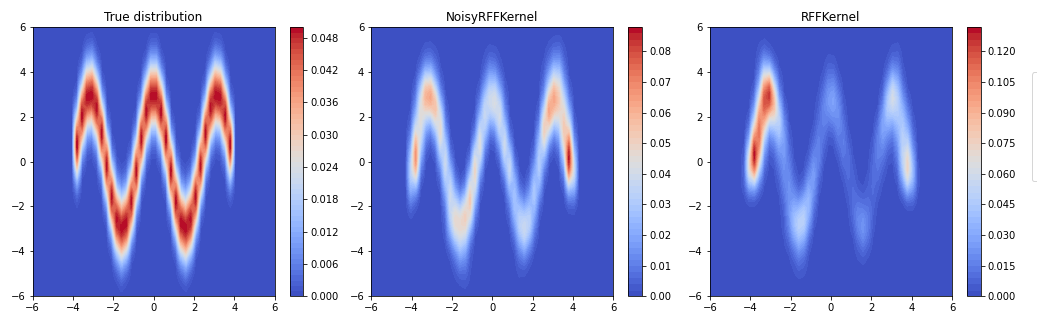
\includegraphics[width=\textwidth]{figures/score_matching/2D/Cosine3500.png}
%       \caption{Cosine}
%     \end{subfigure}

%     \begin{subfigure}[b]{\textwidth}
%       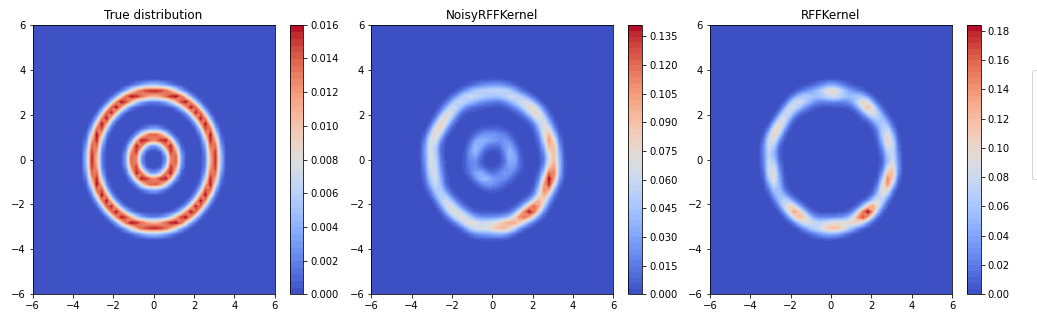
\includegraphics[width=\textwidth]{figures/score_matching/2D/Rings3500.png}
%       \caption{Mixture of rings}
%     \end{subfigure}

%     \caption{Score-matching density estimation using $3500$ sample size for cosine and the mixture of rings deistributions}
%     \label{fig:2d_3500}
% \end{figure}

\begin{figure}[H]
    \centering
    \begin{subfigure}[b]{0.32\textwidth}
        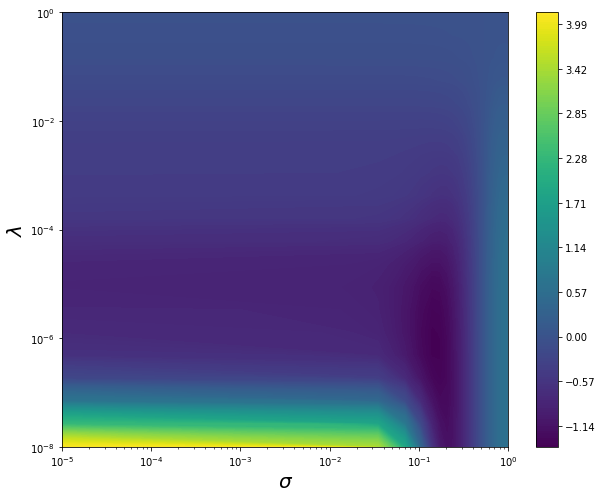
\includegraphics[width=\textwidth]{figures/score_matching/loss/lossCosine.png}
        \caption{Cosine}
    \end{subfigure}
    \begin{subfigure}[b]{0.32\textwidth}
        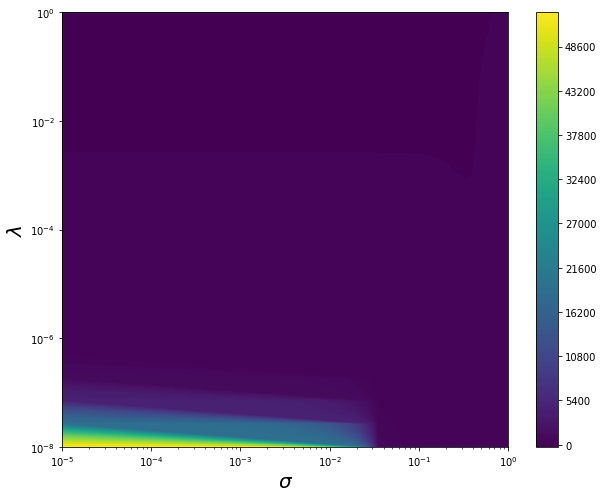
\includegraphics[width=\textwidth]{figures/score_matching/loss/lossBanana.png}
        \caption{Banana}
    \end{subfigure}
    \begin{subfigure}[b]{0.32\textwidth}
        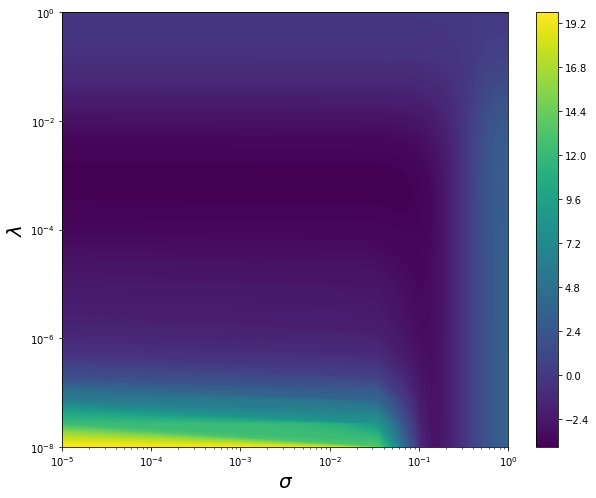
\includegraphics[width=\textwidth]{figures/score_matching/loss/lossRing.png}
        \caption{Ring}
    \end{subfigure}
  \begin{subfigure}[b]{0.32\textwidth}
    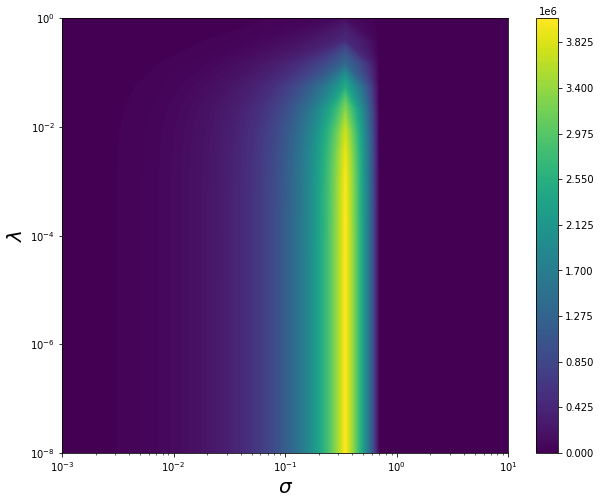
\includegraphics[width=\textwidth]{figures/score_matching/loss/lossMinibone.png}
    \caption{MiniBoone}
  \end{subfigure}
    \begin{subfigure}[b]{0.32\textwidth}
        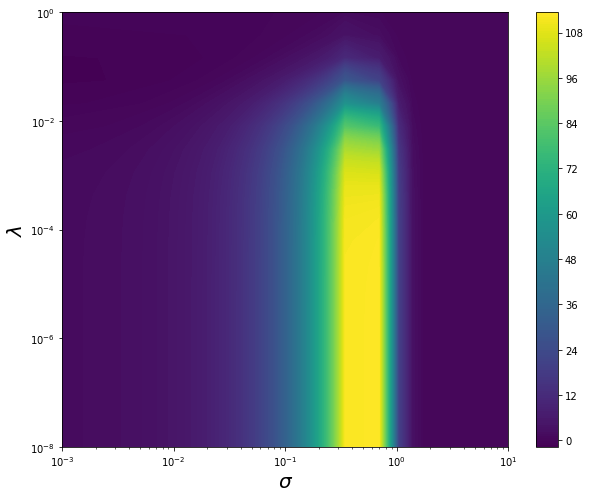
\includegraphics[width=\textwidth]{figures/score_matching/loss/lossRedWine.png}
        \caption{Red Wine}
    \end{subfigure}
    \begin{subfigure}[b]{0.32\textwidth}
        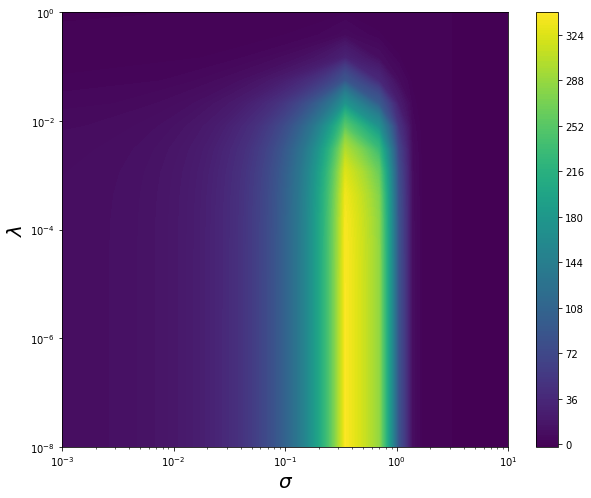
\includegraphics[width=\textwidth]{figures/score_matching/loss/lossWhiteWine.png}
        \caption{White Wine}
    \end{subfigure}
    \caption{Loss surface w.r.t. the regularization parameter $\lambda$ (y axis) and noise parameter $\sigma$ (x axis).}
    \label{fig:lossdemo_app}
\end{figure}

\begin{figure}[H]
    \centering
    \begin{subfigure}[b]{0.8\textwidth}
        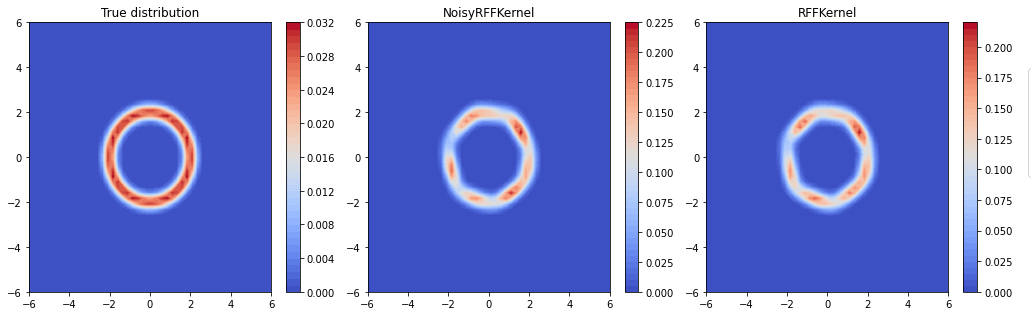
\includegraphics[width=\textwidth]{figures/score_matching/2D/ring1000MOG.png}
        \caption{Ring}
    \end{subfigure}

    \begin{subfigure}[b]{0.8\textwidth}
        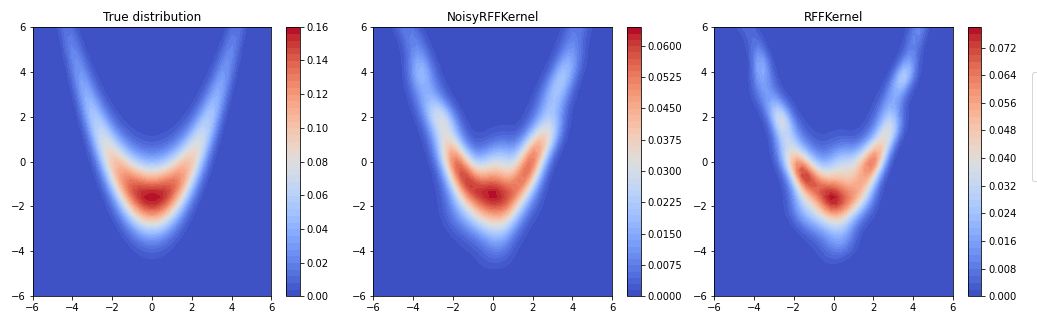
\includegraphics[width=\textwidth]{figures/score_matching/2D/Banana1000.png}
        \caption{Banana}
    \end{subfigure}

    \begin{subfigure}[b]{0.8\textwidth}
        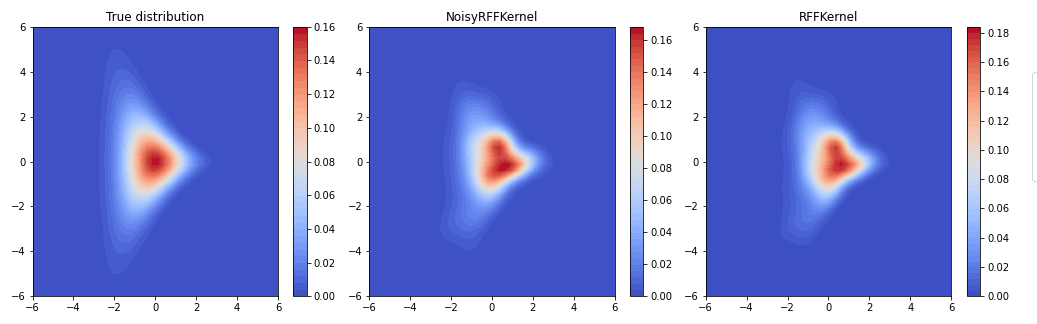
\includegraphics[width=\textwidth]{figures/score_matching/2D/Funnel1000.png}
        \caption{Funnel}
    \end{subfigure}

    \begin{subfigure}[b]{0.8\textwidth}
        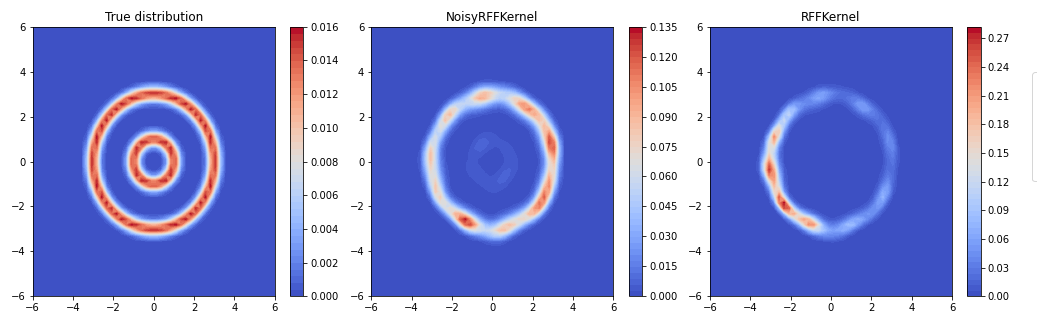
\includegraphics[width=\textwidth]{figures/score_matching/2D/Rings1000.png}
        \caption{Mixture of rings}
    \end{subfigure}

    \begin{subfigure}[b]{0.8\textwidth}
        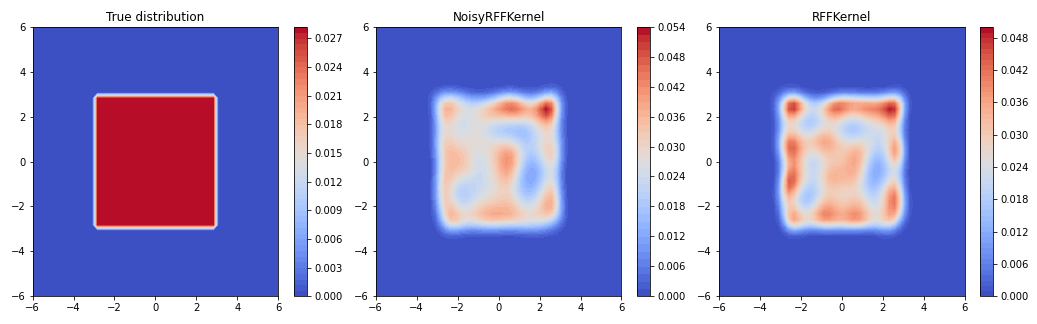
\includegraphics[width=\textwidth]{figures/score_matching/2D/Uniform1000.png}
        \caption{Uniform}
    \end{subfigure}

    \caption{Score-matching density estimation using $1000$ samples.
    The left column is a ground truth, middle is DSM RFf,
    and the right is SM RFF.}
    \label{fig:2d_1000_app}
\end{figure}
